\documentclass[a4paper, 10pt]{article}

\usepackage[russian]{babel}
\usepackage[T2A]{fontenc}
\usepackage[utf8]{inputenc}
\usepackage{multicol}
\usepackage{adjustbox}
\usepackage{amsmath}
\usepackage{tikz}



\usepackage{geometry}
\geometry{top=10mm}
\geometry{bottom=5mm}
\geometry{left=15mm}
\geometry{right=15mm}

\usepackage{graphicx}
\graphicspath{ {./images/} }
\usepackage{wrapfig}

\newcommand{\display}[1]{\hbox to 0.32\textwidth
	{\hfil \small #1 \hfil}}

\newenvironment{ramka}[1]{\begin{flushleft}\begin{tabular}{|p{#1}|}
		\hline}{\\\hline\end{tabular}\end{flushleft}\smallskip}
	
\newcommand{\RomanNumeralCaps}[1]
	{\MakeUppercase{\romannumeral #1}}

\setlength{\parskip}{0pt}

\renewcommand{\a}{\alpha}

\usepackage{fancyhdr}
\pagestyle{empty}


\begin{document}
	\begin{center}
	{\large
	Федеральное государственное автономное образовательное учреждение\\
	высшего образования\\
	«Национальный исследовательский университет ИТМО»
	
	\vspace{5pt}
	Факультет программной инженерии и компьютерной техники
	}
	\vspace{17em}
	
	{\Large Лабораторная работа \textnumero6}\\
	\smallskip
	{\LARGE \textbf{Работа с системой компьютерной вёрстки \TeX}}\\[1em]
	{\large Вариант: 44}
	

\end{center}

\vspace{20em}
{\large
\begin{flushright}
	Выполнил: Состанов Тимур Айратович\\
	Группа: P3114\\
	Преподаватель: Балакшин Павел Валерьевич\
\end{flushright}

\vspace{\fill}

\begin{center}
	Санкт-Петербург
	
	2022г.
\end{center}
}
	\newpage
	\begin{center}
		{\bfseries \Huge Сколько у числа делителей?}\\[3 pt]
		{\large \textsc{Б. КОТЛЯР}}
	\end{center}
	\begin{multicols}{3}
		\rule{0pt}{3.4 em}
		\begin{flushleft}
			\hrule\smallskip
			{\bfseries \large Простое ли число ---\\ единица?}
			\smallskip\hrule\smallskip
		\end{flushleft}
		
		Задумывались ли вы когда-нибудь, почему единицу не принято считать простым числом? Ведь, как и у всякого простого числа, ее делители --- она сама и единица, не так ли?
		
		Разумеется, на то были причины --- не менее веские, чем те, по которым принято считать параллельными совпадающие прямые. Если исключить их из числа параллельных, приходится во множестве формулировок геометрических фактов рассматривать возможность совпадения двух прямых отдельно, хотя теоремы и аксиомы без изъятий распространяются на этот случай.
		
		Единица, долго причислявшаяся к простым числам, лишилась этого звания из сугубо практических соображений. Очень удобно было бы, чтобы разложение всякого натурального числа на простые множители было единственным, но если считать, что
		число 1 простое, справедливость этого
		утверждения нарушается.
		
		Разложим для примера на простые множители какое-нибудь число, скажем, 84:\\
		\display{$84 = 2 \cdot 2 \cdot 3 \cdot 7 = 2^2 \cdot 3 \cdot 7$}
		Можно ли разложить его как-то иначе? Разумеется, можно переставлять
		сомножители местами, нотакие разложения естественно считать совпадающими. То, что других разложений нет,вытекает из так называемой «основной теоремы арифметики», утверждающей, что \textit{любое натуральное число разлагается на простые множители, причем (с точностью до перестановхи) единственным образом}, т.е. натуральное число N однозначно представляется в виде
		\display{$N = p_1^{\a_1}p_2^{\a_2}\ldots p_k^{\a_k}$}
		где $p_1, \ldots, p_k$ -- разные простые числа, a $\a_1, \ldots, \a_k$ -- натуральные числа.
		
		Вернемся к нашему примеру. Число 2 входит в разложение числа 84 во второй степени, 3 и 7 -- в первой. А в какой степенивходит в разложение
		
		
		\columnbreak
		
		\begin{ramka}{0.296\textwidth}
			\\
			\textit{\large Пробороненные просторы} \\
			\textit{\large Так гладко улеглись вдали,}\\
			\textit{\large Как будто выровняли горы}\\
			\textit{\large Или равнину подмели.} \\[3 pt]
			\hbox to 5.2cm {\hfil Б. Пастернак}
		\end{ramka}
	
		\noindent
		 этого числа простой множитель 5? Ни в какой, т.е. внулевой. Так что можно
		 считать, что в разложении содержатся все простые числа, но некоторые — в
		 нулевой стелени. Конечно, мы будем в дальнейшем выписывать только те
		 сомножители, которые входят в разложение «по-настоящему».
		 
		 Теперь понятно, почему неудобно считать 1 простым числом. Ведь ее
		 можно приписать к разложению множителем в любой степени:

		\display{$84 = 1^5 \cdot 2^2 \cdot 3 \cdot 7 = 1^{100} \cdot 2^2 \cdot 3 \cdot 7$}
		\noindent
		и т.д. Тем самым единственность разложения на простые множители оказалась потерянной.
		
		Есть еще ряд причин — и простых, и довольно хитрых — в пользу того,
		чтобы единицу простым числом не считать. Напишем подряд несколько
		первых натуральных чисел, а под ними — число их делителей (учитывая
		только различные делители каждого числа). Для числа $N$ числоего делите-
		лей обозначим $\tau(N)$. Из получившейся таблицы видно, что уединицы лишь один делитель; у всех остальных натуральных чисел их больше (причем у
		простых -- ровно по два). Поэтому желательно выделить её в отдельный
		класс чисел — и не простых, и не составных.
		
		\bigskip
		\hrule\smallskip
		{\bfseries \large \noindent Число делителей\\ натурального числа}
		\smallskip\hrule\smallskip

		Можно ли записать функцию $\tau(N)$ аналитически? Оказывается, можно,
		и даже не очень сложно. Давайте посмотрим, как это делается.
		
		Будем записывать натуральное число $N$ виде произведения тех простых, которые в ненулевой степени
		
		\rule{0pt}{4 em}

		\begin{adjustbox}{width=0.66\textwidth}
			\begin{tabular}{|c|c|c|c|c|c|c|c|c|c|c|c|c|}
				\hline
				{\footnotesize $N$} & {\footnotesize 1} & {\footnotesize 2} & {\footnotesize 3} & {\footnotesize 4} & {\footnotesize 5} & {\footnotesize 6} & {\footnotesize 7} & {\footnotesize 8} & {\footnotesize 9} & {\footnotesize 10} & {\footnotesize 11} & {\footnotesize 12}\\
				\hline
				{\footnotesize $\tau \left( N \right)$} & {\footnotesize 1} & {\footnotesize 2} & {\footnotesize 2} & {\footnotesize 3} & {\footnotesize 2} & {\footnotesize 4} & {\footnotesize 2} & {\footnotesize 4} & {\footnotesize 3} & {\footnotesize 4} & {\footnotesize 2} & {\footnotesize 6}\\
				\hline
			\end{tabular}
		\end{adjustbox}
				
		\columnbreak
		\rule{0pt}{3.57 em}
		
		\noindent
		входят в разложение этого числа. Рассмотрим, как и раньше, равенство\\
		\display{$N = p_1^{\a_1} p_2^{\a_2} \ldots p_k^{\a_k}$}
		с различными простыми $p_1, p_2, \ldots, p_k$ и натуральными показателями  $\a_1, a_2, \ldots, \a_k$. (Такое представление называется \textit{каноническим разложениеем} числа $N$.)
		
		\textbf{Теорема. }\textit{Если}\\
		\display{$N = p_1^{\a_1} p_2^{\a_2} \ldots p_k^{\a_k}$ --} 
		\textit{каноническое разложение натурального числа $N$, то}
		\medskip
		
		\display{$\tau(N) = \left(\a_1 + 1\right)\left(\a_2 + 1\right)\ldots\left(\a_k + 1\right)$}
		\medskip
		
		\textbf{Доказательство.} Любой положительный делитель числа $N$ имеет вид $p_1^{\beta_1} p_2^{\beta_2} \ldots p_k^{\beta_k}$, где $0\leq\beta_1\leq\a_1,$ $0\leq\beta_ 2\leq\a_2,\ldots, 0\leq\beta_k\leq\a_k$. Например, если все $\beta_i = 0$, то делитель равен 1, если все $\beta_i = \a_i$, то делитель равен $N$. Сколько же таких делителей можно образовать? Показатель $\beta_1$ принимает ровно $\a_1 + 1$ значений --- $0, 1, 2, \ldots, \a_1$; $\beta_2$ принимает $\a_2 + 1$ значений и т.д. Поэтому различных делителей вида $p_1^{\beta_1}$ будет $\a_1 + 1$, делителей вида $p_2^{\beta_2}$ будет $\a_2 + 1$; следовательно делителей вида $p_1^{\beta_1}p_2^{\beta_2}$ будет ровно $\left(\a_1 + 1\right) \left(\a_2 + 1\right)$. Продолжая этот процесс дальше, получим требуемый результат.\\
		
		Пользуясь этой формулой, можно найти число делителей любого натурального числа, но сначала придется разложить это число на множители, чтобы узнать показатели $\a_1, a_2, \ldots, \a_k$. А это не всегда просто сделать: ведь для очень большого числа трудно понять, простое оно или составное, тем более -- написать его каноническое разложение.\\
		
		Это не единственный недостаток приведенной формулы. Поведение функции $\tau(N)$ хаотично: с одной стороны, для каждого числа
		
		\rule{0pt}{2.7em}
		
		\hbox to 0.565\textwidth
			{\hfil \textsl{Таблица}\hfil}
		
		

	\end{multicols}

	\noindent
	\hbox to 0.5\textwidth {\small $4^*$\hss 15}

	
	\newpage
	
	\hbox to 0.585\textwidth {\small 16\hss \textmd{КВАНТ} $\cdot$ $1994$ $  \slash$ \textnumero  4}
	\begin{multicols*}{3}
		\rule{0pt}{0.6 \textheight}
		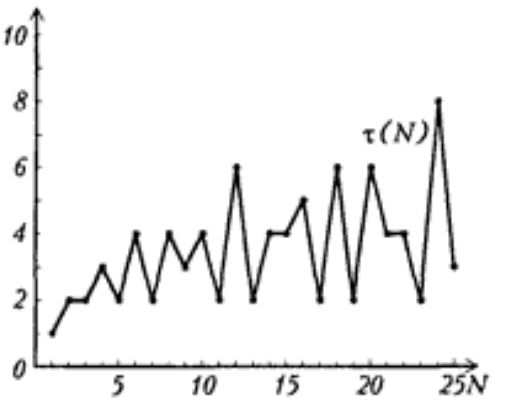
\includegraphics[width=\columnwidth]{pict}
		\hbox to 0.13\textwidth
		{\hfil \textsl{Рис. 1}\hfil}
	
		\columnbreak
		\rule{0pt}{0.2 \textheight}
		
		{\footnotesize
		\begin{multline*}
			\tau(N) = \tau(2^n) = n + 1 = \log_2 N + 1 =\\
			= \log_2 N + \log_2 2 = \log_2 {(2N)}.
		\end{multline*}
		}
	
	\end{multicols*}

	\newpage
	\begin{center}
		{\large \textsc{Дополнительное задание}}
	\end{center}
	\[f(x,y,\a,\beta) = \frac{\sum\limits_{n=1}^{\infty} A_n \cos {\left(\frac{2 n \pi x}{\a}\right)}}{\prod \mathcal{F} g(x, y)}
	\]
	
    \newpage
    \begin{minipage}{0.3\textwidth}
    	\rule{0pt}{30 em}
    	\begin{tikzpicture}[scale=1.6, line width=2pt]
    		\filldraw[orange] (1.7,0) -- (1.7,0.5) arc (90:0:1.4 em);
    		\filldraw[yellow] (1.7,0) -- (1.7,0.5) arc (90:180:1.4 em);
    		\draw[blue] (1.7,0) -- (1.7,3);
    		\draw[dashed, orange] (0,0) -- (1.7,3);
    		\draw[dashed, black] (0,0) -- (1.7,0);
    		\draw[orange] (3.4,0) -- (1.7,3);
    		\draw[black] (1.7,0) -- (3.4,0);
    		\node[below left] at (0,0) {D};
    		\node[below right] at (3.4,0) {C};
    		\node[below] at (1.7,0) {A};
    		\node[above] at (1.7,3) {B};
    	\end{tikzpicture}
    \end{minipage}
	\hfil
    \begin{minipage}{0.55\textwidth}
    	{\hfil \Large $74$\hspace*{1.6 em} КНИГА \RomanNumeralCaps{1} ПРЕДЛ. \RomanNumeralCaps{48}. ТЕОРЕМА}
    	\vspace*{1.6 em}
    	\begin{wrapfigure}{l}{0.2\textwidth}
    		
\includegraphics[width=0.2\textwidth]{E}
    	\end{wrapfigure}
	\phantom{Я ненавижу Latex}\\
	\textit{\large сли в треугольнике квадрат одной стороны }
	\begin{tikzpicture}
		\draw[ultra thick, orange] (0,0) -- (1.3,0);
		\node[above left] at (0.3,0) {\scriptsize B};
		\node[above right] at (1,0) {\scriptsize C};
	\end{tikzpicture}
	\textit{\large равен сумме квадратов двух других сторон}

    \end{minipage}

	
\end{document}